\documentclass[a4paper,12pt]{article}
\usepackage{graphicx}
\usepackage{color}
\usepackage{transparent}

\addtolength{\oddsidemargin}{-1in}
\addtolength{\evensidemargin}{-1in}
\addtolength{\topmargin}{-1in}
\addtolength{\textwidth}{2in}
\addtolength{\textheight}{2in}

\begin{document}

\section*{VNS Quick Start Guide}

VNS is a network simulator running on a server in the computer lab.  It lets you get round the problems associated with testing networking programs on your own machine, such as lack of internet when anything goes wrong.  VNS also lets you create your own virtual networks which can be configured as desired.

\subsection*{How VNS works}
A VNS network is known as a topology.  There are usually many topologies active simultaneously on the VNS server; you will have your own topology which only you have access to.

A topology will typically have several nodes, each connected to several other nodes.  When you run a program that interacts with a VNS topology, it runs on your own computer or workstation.  The VNS server sends your program packets which your program's node is meant to receive, and your program can send packets to the VNS server to be sent to one of the other nodes in the topology.

Most topologies have a gateway, which allows them to send and receive packets to and from the outside world.\footnote{Some topoogies might be allocated IP addresses in a private block, e.g. 10.0.0.0/8, which prevent them receiving packets from outside the local network.  Some topologies might also have IP filters, so only some IP addresses can send packets into the topology.}  This lets you send and receive packets to and from the topology from the machine you're working on, as if the topology were a set of real machines.  This is independent of the way your program connects to the VNS server.

As an example, consider the following situation:

\mbox{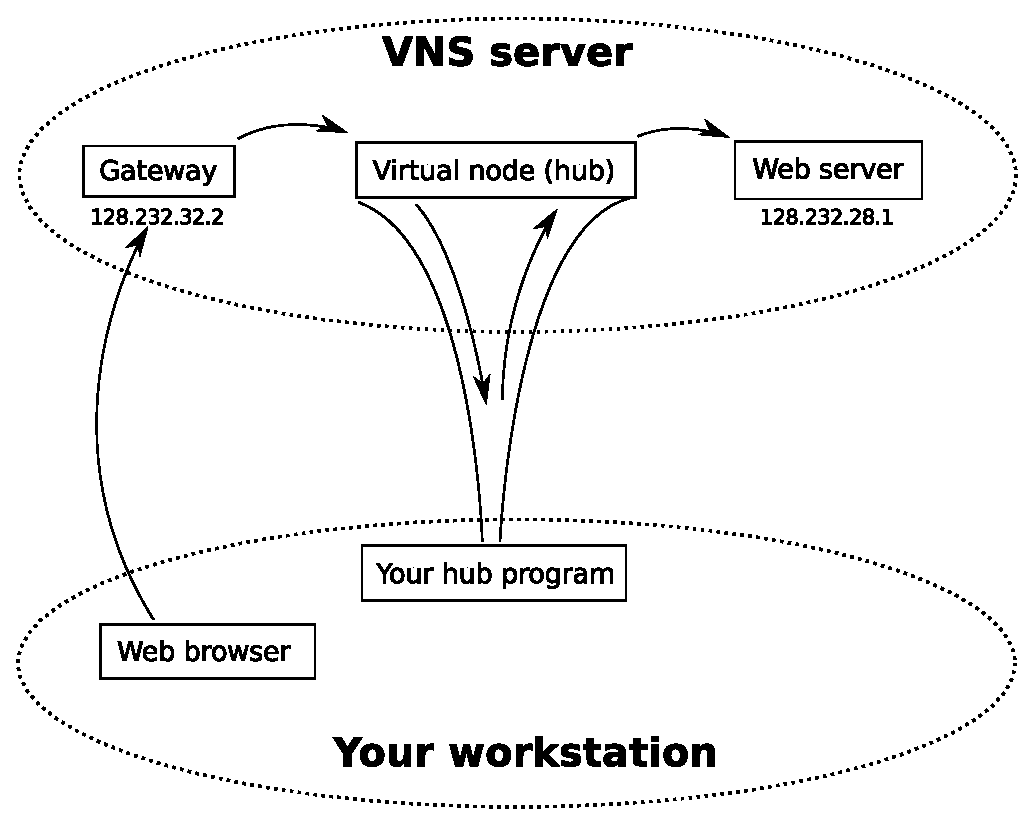
\includegraphics[width=300pt]{example.eps}}

Your program running on your work station is connected to the VNS server and takes the place of the virtual node.  A web browser running separately on your workstation sends a TCP SYN request to the web server, and it is received by the gateway, which sends it to the virtual node.  The VNS server recognises that your program should be dealing with packets sent to the virtual node, and sends it to your program back on your workstation.  Your program then sends it it back to the VNS server with instructions to send it on to the webserver.\footnote{For simplicity, this ignores details like ARP packets.}

\subsection*{Writing programs to use VNS}
You will be provided with a library or stub code which handles all communication with VNS itself, leaving you free to concentrate on the networking assignment rather than the details of VNS.

\end{document}
